\documentclass[landscape,final,a0paper,fontscale=0.277]{baposter}

\usepackage{graphicx}
\usepackage{url}
\usepackage{multicol}
\usepackage{enumitem}
\usepackage{bm}
\usepackage{relsize}
\usepackage{multirow}
\usepackage{rotating}

%\setlength{\columnsep}{1.5em}
%\setlength{\columnseprule}{0mm}

\graphicspath{{images/}{./images/}}


\definecolor{darkblue}{HTML}{0000FF}
\definecolor{lightblue}{HTML}{00AAAA}
\definecolor{lightestblue}{HTML}{00FFFF}

\hyphenation{resolution occlusions}

\newcommand{\compresslist}{%
\setlength{\itemsep}{1pt}%
\setlength{\parskip}{0pt}%  
\setlength{\parsep}{0pt}%
}

\begin{document}

\begin{poster}
{
	grid = false,
	columns=3,
	bgColorOne = lightestblue,
	borderColor = lightblue,
	headerColorOne = white,
	headerFontColor = black,
	boxColorOne = white,
	textborder = rounded,
	eyecatcher = true,
	headerborder = closed,
	headerheight = 0.1\textheight,
	headershape = smallrounded,
	headershade = plain,
	headerfont =  \Large\bf\textsc,
	textfont = {\setlength{\parindent}{1.5em}},
	boxshade = plain,
	background = plain,
	linewidth = 2pt
}
{
\includegraphics[height=4em]{./images/logo}}
{\bf\textsc{Desert Fox: a Simple Wargame AI}\vspace{0.5em}}
{\textsc{Parker Michaleson}}
{
\includegraphics[height=4em]{./images/logo}}

\headerbox{Introduction}{name=introduction, column=0, row=0}
{
Playing wargames, ranging from classics like Chess to Go to modern consumer games like Total War, presents a historically interesting problem for AI researchers. Much progress has been made on the front of playing Chess and similar games with small search spaces and simple heuristics by using traditional search techniques. Games with large search spaces which lack good heuristics, like Go, however, have presented a major challenge for such techniques. Here we demonstrate the method of the {\it Monte Carlo Tree Search} for playing a simple game derived from the commercial game Memoir '44 called Desert Fox which, like Go, possesses a large search space and lacks search heuristics.
}

\headerbox{General Strategy}{name=strategy, column=1, row=0}
{
Desert Fox possesses a large search space compared to other games due to its simple, unrestrictive, rules, on any given turn, a player may order at least one and up to four of his/her units. An order to the unit consists of up to two tiles of movement and one combat instruction. In addition, Desert Fox uses hexagonal tiles, all of which are passable to the unit unless occupied by an enemy unit. Then for any given unit, the number of possible orders during a turn consists of at least 19 possible moves {\it without considering combat}. On the picture below, we can see the range for movement with combat in red, the range for maximum movement in yellow, and the maximum combat range in green.

\center{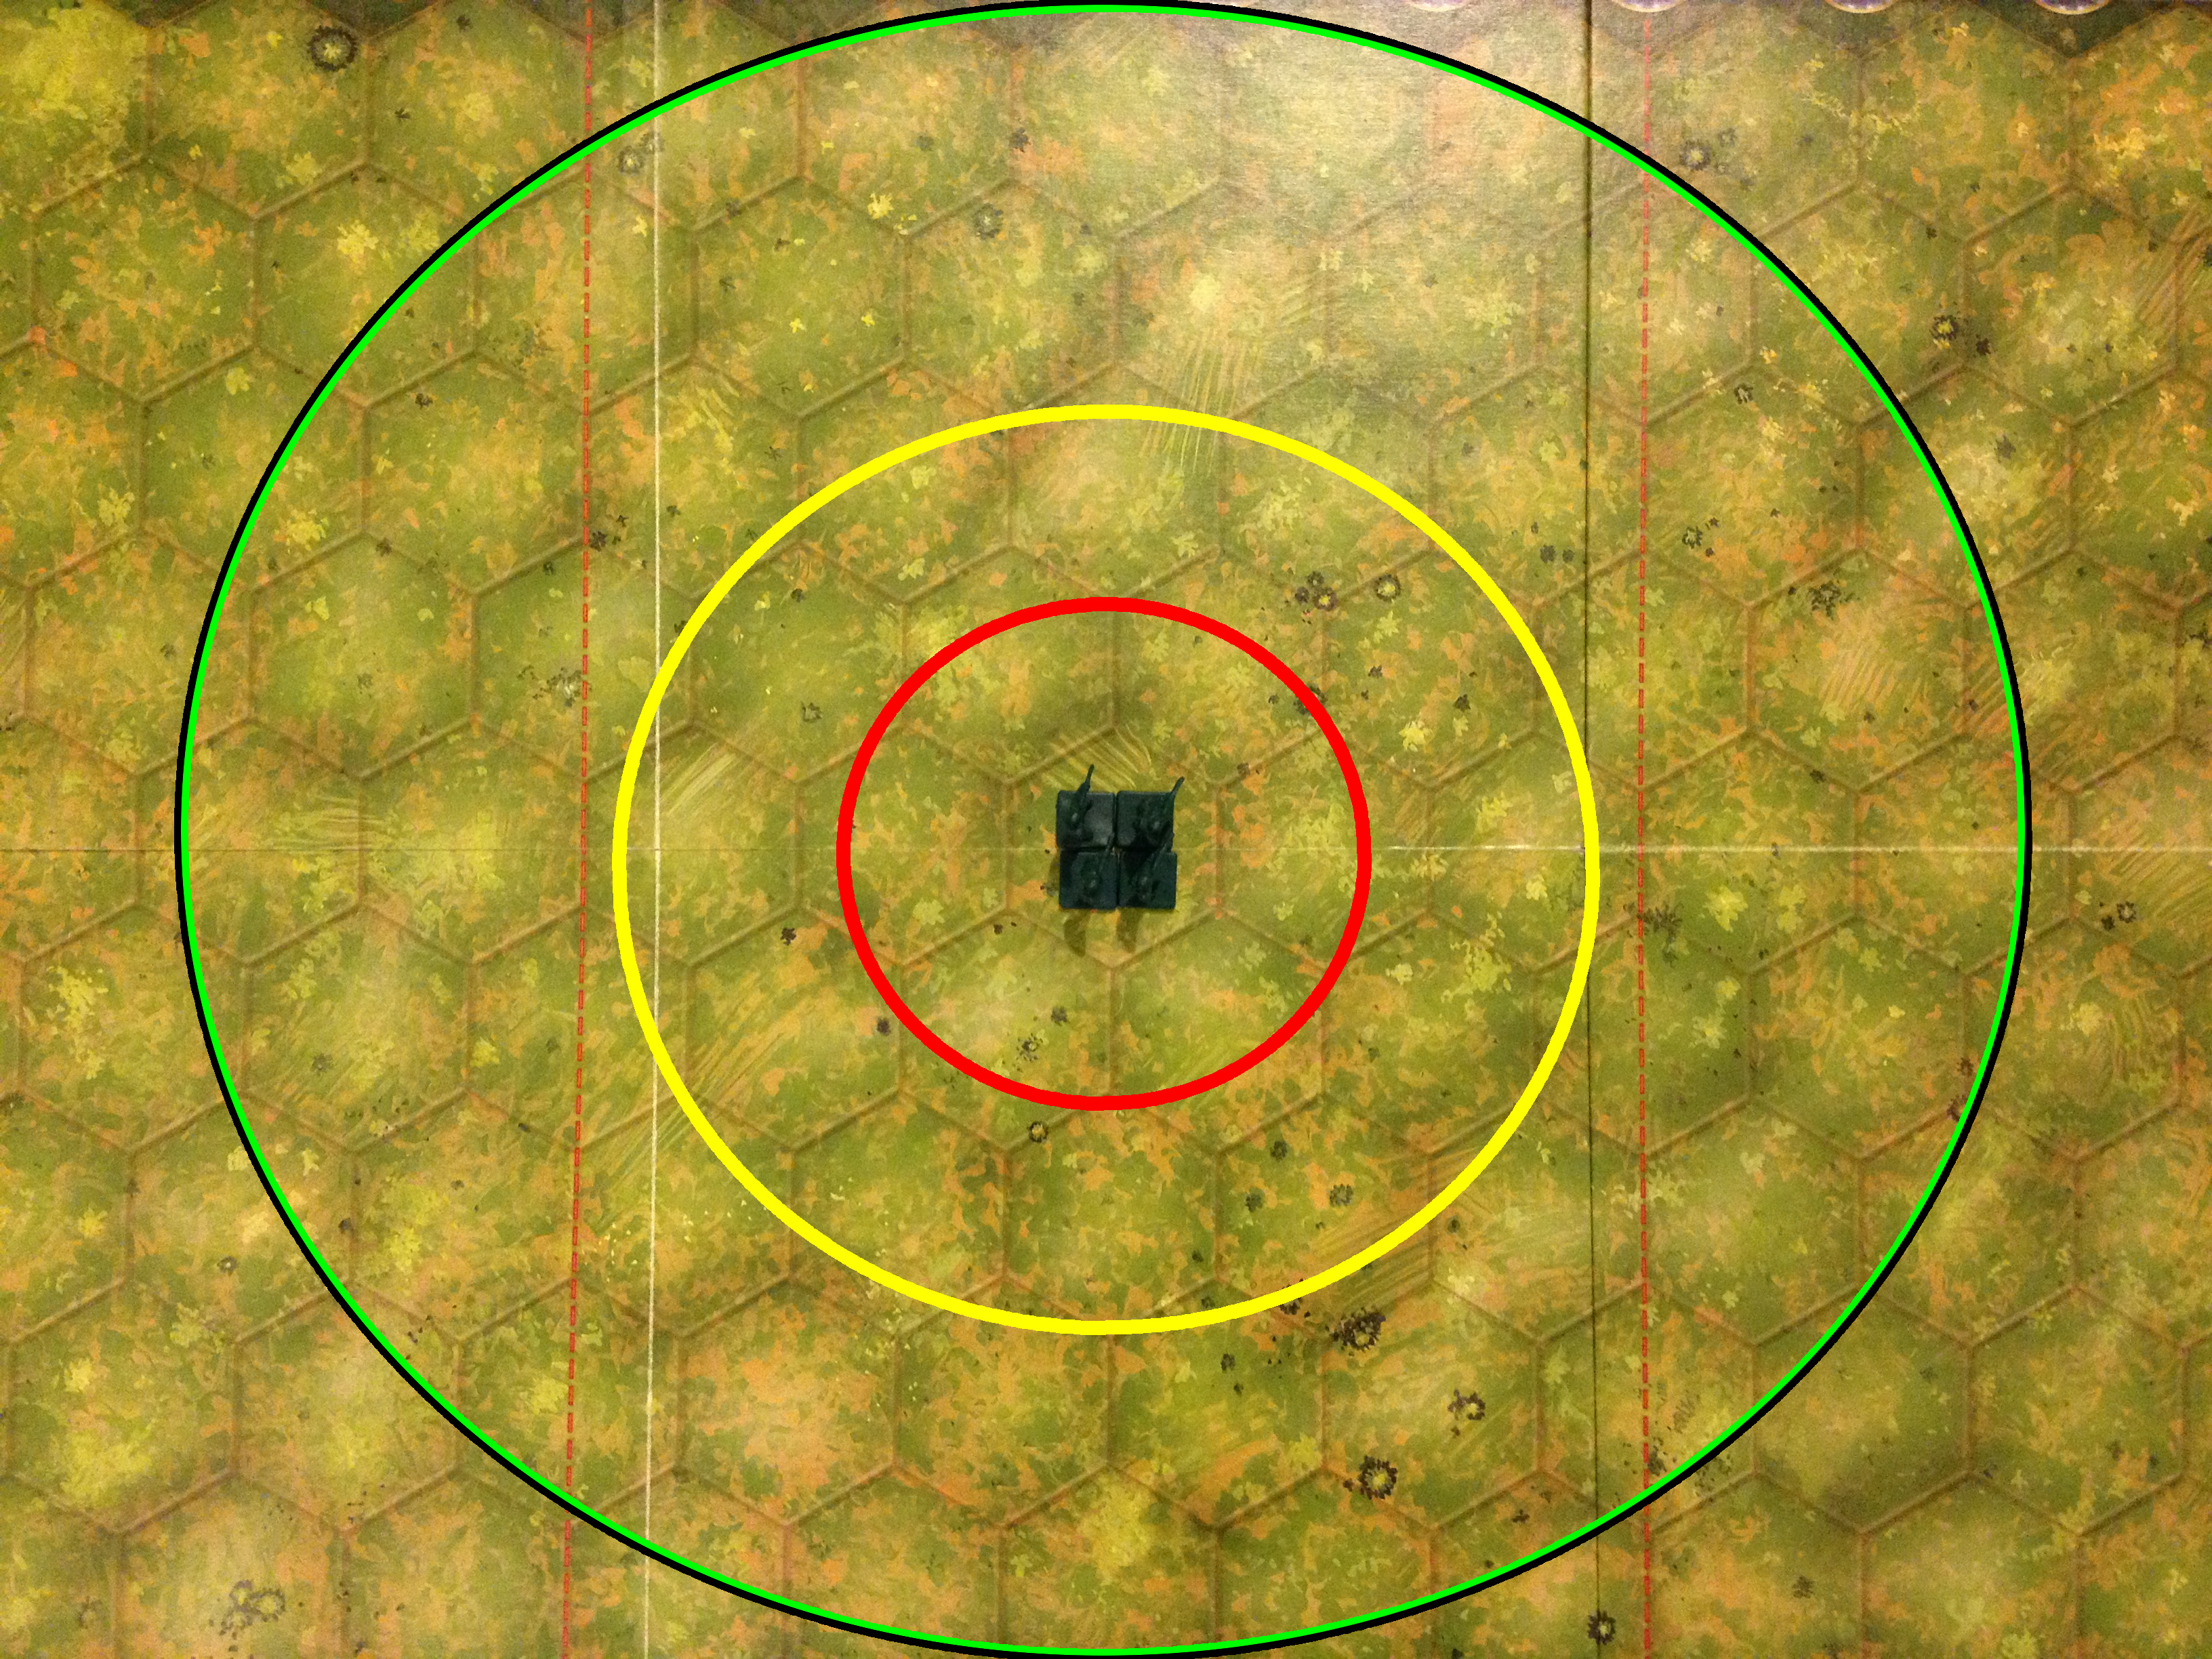
\includegraphics[width=25em]{images/ranged_board.png}}

To add to the complexity, the player must often choose units to order out of a pool of a dozen or more units based on cards in the player's hand. This leads to a swiftly growing combinatoric problem with an unreasonable size for a traditional unguided search and a lack of clear cut heuristics for implementing a guided search. This project works around traditional limitations by using the Monte Carlo Tree Search (MCTS), which uses a large sampling of child states to find a close-to-optimal action for a given parent state. MCTS can be further improved by adding a heuristic to opportunistically probe promising child states which are likely to be close-to-optimal. While there exists no simple heuristic rule for this game, we can use a learning technique such as Q-Learning to generate a heuristic by observing gameplay and adjusting the heuristic function accordingly.
}

\headerbox{Conclusions}{name=conclusions, column=2, row=0}
{
}

\headerbox{References}{name=references, column=2, below=conclusions}
{
Some major works useful to this project are given below:

\begin{thebibliography}{9}

  \bibitem{amato10}
  High-level Reinforcement Learning in Strategy Games. Christopher Amato and Guy Shanai. {\it Proc. of 9\textsuperscript{th} Int. Conf. on Autonomous Agents and Multiagent Systems (AAMAS 2010).}

  \bibitem{brown09}
  A Survey of Mente Carlo Tree Search Methods. Browne, Powley, {\it et. al.}. {\it IEEE Transactions of Computational Intelligence and AI in Games, Vol. 4, No. 1, MARCH 2012.}

\end{thebibliography}
}

\headerbox{Source Code}{name=source, column=2, below=references}
{
The source code is available as a Git repository at:

\indent{    } \url{github.com/pcm2718/psychic-pikeman.git}
}

\end{poster}

\end{document}
